% Divide and Conquer Part 3 -- Metropolis beamer slides
% Compile: pdflatex divide-and-conquer-3.tex (x2)
\documentclass[10pt,aspectratio=169]{beamer}

\usetheme{metropolis}
\metroset{block=fill, numbering=fraction, progressbar=frametitle}

\usepackage[T1]{fontenc}
\usepackage{amsmath, amssymb}
\usepackage{listings}
\usepackage{booktabs}
\usepackage{tikz}
\usepackage{pgfplots}
\pgfplotsset{compat=1.18}
\usetikzlibrary{arrows.meta, positioning, decorations.pathreplacing, calc}

% ---- colors -------------------------------------------------------------
\definecolor{mLightBlue}{HTML}{4C72B0}
\definecolor{mGreen}{HTML}{55A868}
\definecolor{mRed}{HTML}{C44E52}
\definecolor{mGray}{HTML}{BFBFBF}
\setbeamercolor{alerted text}{fg=mRed}

% ---- code style ---------------------------------------------------------
\lstdefinestyle{jl}{
  basicstyle=\ttfamily\footnotesize,
  keywordstyle=\color{mRed}\bfseries,
  commentstyle=\color{mGreen}\itshape,
  numberstyle=\tiny\color{mGray},
  showstringspaces=false,
  breaklines=true,
  columns=fullflexible,
  morekeywords={function,for,in,if,else,elseif,end,return,length,while,nothing,sort}
}
\lstset{style=jl}

% ---- title --------------------------------------------------------------
\title{Divide and Conquer, Part 3}
\subtitle{Karatsuba's Algorithm, Linear Time Selection}
\date{}
\author{}

\begin{document}

\maketitle

% =========================================================================
\section{Karatsuba's Algorithm}

\begin{frame}{Multiplying Big Integers}
  Multiplying two 32- or 64-bit integers is a single hardware instruction.

  \bigskip
  But for integers with \alert{millions of digits}, the grade-school algorithm's $O(n^2)$ starts to hurt.

  \bigskip
  \begin{center}
  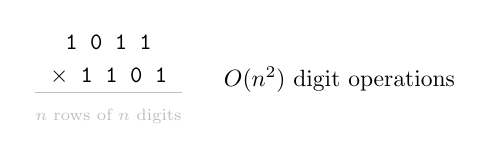
\begin{tikzpicture}[scale=0.85, every node/.style={transform shape}]
    \node at (0,0) {\ttfamily 1 0 1 1};
    \node at (0,-0.5) {\ttfamily $\times$ 1 1 0 1};
    \draw[mGray] (-1.1,-0.75) -- (1.1,-0.75);
    \node[mGray] at (0,-1.1) {\scriptsize $n$ rows of $n$ digits};
    \node[right] at (1.6,-0.55) {$O(n^2)$ digit operations};
  \end{tikzpicture}
  \end{center}

  \bigskip
  \begin{center}
    Can we do better?
  \end{center}
\end{frame}

\begin{frame}{Splitting the Inputs}
  Write each $n$-bit number as a high half and a low half, with $m = \lfloor n/2 \rfloor$:
  \[
    x = x_1 \cdot 2^m + x_0,
    \qquad
    y = y_1 \cdot 2^m + y_0.
  \]

  \bigskip
  \begin{center}
  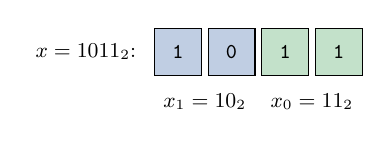
\begin{tikzpicture}[scale=0.85, every node/.style={transform shape}]
    \foreach \v [count=\i from 0] in {1,0,1,1} {
      \ifnum\i<2 \def\fillc{mLightBlue!35}\else\def\fillc{mGreen!35}\fi
      \node[draw, minimum size=7mm, fill=\fillc] at (\i*0.8,0) {\small \tt \v};
    }
    \node[left] at (-0.5,0) {\small $x = 1011_2$:};
    \node[below] at (0.4,-0.5) {\small $x_1 = 10_2$};
    \node[below] at (2.0,-0.5) {\small $x_0 = 11_2$};
  \end{tikzpicture}
  \end{center}

  \bigskip
  Expanding directly:
  \[
    x \cdot y = x_1 y_1 \cdot 2^{2m} + (x_1 y_0 + x_0 y_1)\cdot 2^m + x_0 y_0.
  \]
\end{frame}

\begin{frame}{The Naive Split Gains Nothing}
  That expansion needs \alert{four} half-size multiplications:
  \[
    x_1 y_1, \quad x_1 y_0, \quad x_0 y_1, \quad x_0 y_0.
  \]

  \bigskip
  Additions and shifts are $O(n)$, so
  \[
    T(n) = 4\,T(n/2) + O(n)
    \;\overset{\text{Master}}{=}\; O(n^2).
  \]

  \bigskip
  \begin{center}
    Exactly what we started with.
  \end{center}
\end{frame}

\begin{frame}{Karatsuba's Trick}
  The middle coefficient needs only \alert{one} extra multiplication. Define
  \[
    P_1 = x_1 y_1, \qquad P_2 = x_0 y_0, \qquad P_3 = (x_1 + x_0)(y_1 + y_0).
  \]

  \bigskip
  Then
  \[
    x_1 y_0 + x_0 y_1 = P_3 - P_1 - P_2,
  \]
  and therefore
  \[
    x \cdot y = P_1 \cdot 2^{2m} + (P_3 - P_1 - P_2)\cdot 2^m + P_2.
  \]

  \bigskip
  \begin{center}
    \alert{Three} multiplications instead of four.
  \end{center}
\end{frame}

\begin{frame}{Exercise}
  \begin{center}
    Verify that $P_3 - P_1 - P_2 = x_1 y_0 + x_0 y_1$ by expanding $P_3$.
  \end{center}
\end{frame}

\begin{frame}{Solution}
  Expand the product:
  \[
    P_3 = (x_1 + x_0)(y_1 + y_0)
        = \underbrace{x_1 y_1}_{P_1} + x_1 y_0 + x_0 y_1 + \underbrace{x_0 y_0}_{P_2}.
  \]

  \bigskip
  Subtracting $P_1$ and $P_2$ leaves exactly the middle terms:
  \[
    P_3 - P_1 - P_2 = x_1 y_0 + x_0 y_1. \qquad \square
  \]

  \bigskip
  \begin{center}
    \small We trade one multiplication for a few extra additions, which is a good deal,
    since additions are only $O(n)$.
  \end{center}
\end{frame}

\begin{frame}{Running Time}
  Three half-size multiplications plus $O(n)$ of additions and shifts:

  \begin{alertblock}{}
    \[
      T(n) = 3\,T(n/2) + O(n)
    \]
  \end{alertblock}

  \bigskip
  Master theorem with $a = 3$, $b = 2$, $d = 1$. Since $\log_2 3 \approx 1.585 > 1$:
  \[
    T(n) = O(n^{\log_2 3}) \approx O(n^{1.585}).
  \]

  \bigskip
  \begin{center}
    A real improvement over $O(n^2)$ for large $n$.
  \end{center}
\end{frame}

\begin{frame}[fragile]{Implementation}
  \begin{lstlisting}
function karatsuba(x::BigInt, y::BigInt)
    # Base case: built-in multiplication for small numbers
    if x < 4 || y < 4
        return x * y
    end

    n = max(ndigits(x, base=2), ndigits(y, base=2))
    m = n div 2

    # Split x = x1 * 2^m + x0,  y = y1 * 2^m + y0
    x1, x0 = x >> m, x & ((BigInt(1) << m) - 1)
    y1, y0 = y >> m, y & ((BigInt(1) << m) - 1)

    # Three recursive multiplications
    P1 = karatsuba(x1, y1)
    P2 = karatsuba(x0, y0)
    P3 = karatsuba(x1 + x0, y1 + y0)

    return (P1 << 2m) + ((P3 - P1 - P2) << m) + P2
end
  \end{lstlisting}
\end{frame}

% =========================================================================
\section{Linear Time Selection}

\begin{frame}{The Selection Problem}
  Given an \alert{unsorted} array $A[1:n]$ and $k$, find the $k$-th smallest element.

  \bigskip
  \begin{center}
  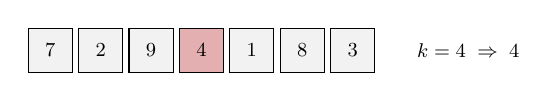
\begin{tikzpicture}[scale=0.8, every node/.style={transform shape}]
    \foreach \v [count=\i from 0] in {7,2,9,4,1,8,3} {
      \ifnum\i=3 \def\fillc{mRed!45}\else\def\fillc{black!5}\fi
      \node[draw, minimum size=7mm, fill=\fillc] at (\i*0.8,0) {\small \v};
    }
    \node[right] at (5.7,0) {\small $k = 4 \;\Rightarrow\; 4$};
  \end{tikzpicture}
  \end{center}

  \bigskip
  \begin{itemize}
    \item $k = 1$: the minimum \quad $k = n$: the maximum
    \item $k = \lceil n/2 \rceil$: the median
  \end{itemize}

  \bigskip
  \begin{center}
    Sorting gives $O(n \log n)$. Can we do better?
  \end{center}
\end{frame}

\begin{frame}{Quickselect}
  Pick a \alert{pivot} $p$ and partition:

  \bigskip
  \begin{center}
  
\begin{tikzpicture}[scale=0.9, every node/.style={transform shape}]
    \fill[mLightBlue!30, draw=mLightBlue] (0,0) rectangle (3.0,0.7);
    \fill[mRed!40, draw=mRed]             (3.0,0) rectangle (3.9,0.7);
    \fill[mGreen!30, draw=mGreen]         (3.9,0) rectangle (7.5,0.7);
    \node at (1.5,0.35) {\small $L$ ($< p$)};
    \node at (3.45,0.35) {\small $E$};
    \node at (5.7,0.35) {\small $G$ ($> p$)};
  \end{tikzpicture}
  \end{center}

  \bigskip
  \begin{itemize}
    \item $k \le |L|$: \; recurse into $L$.
    \item $k \le |L| + |E|$: \; the answer is $p$.
    \item otherwise: \; recurse into $G$ looking for the $(k - |L| - |E|)$-th smallest.
  \end{itemize}

  \bigskip
  \begin{center}
    \small Only \alert{one} side is searched, unlike quicksort.
  \end{center}
\end{frame}

\begin{frame}[fragile]{Quickselect}
  \begin{lstlisting}
function quickselect(A, k)
    n = length(A)
    if n == 1
        return A[1]
    end

    p = A[rand(1:n)]  # random pivot

    L = [a for a in A if a < p]
    E = [a for a in A if a == p]
    G = [a for a in A if a > p]

    if k <= length(L)
        return quickselect(L, k)
    elseif k <= length(L) + length(E)
        return p
    else
        return quickselect(G, k - length(L) - length(E))
    end
end
  \end{lstlisting}
\end{frame}

\begin{frame}{Quickselect: Expected Time}
  With probability $1/2$ the random pivot lands between the $n/4$-th and $3n/4$-th smallest,
  so both $L$ and $G$ have at most $3n/4$ elements.

  \bigskip
  \begin{center}
  
\begin{tikzpicture}[scale=0.9, every node/.style={transform shape}]
    \fill[black!8] (0,0) rectangle (8,0.6);
    \fill[mGreen!35] (2,0) rectangle (6,0.6);
    \draw[mGray] (0,0) rectangle (8,0.6);
    \node at (4,0.3) {\small good pivot};
    \node[below] at (2,-0.1) {\scriptsize $n/4$};
    \node[below] at (6,-0.1) {\scriptsize $3n/4$};
  \end{tikzpicture}
  \end{center}

  \bigskip
  In expectation the size shrinks by $3/4$ every couple of calls:
  \[
    T(n) = T(3n/4) + O(n) \;=\; O(n).
  \]

  \bigskip
  \begin{center}
    \small Expected $O(n)$, but the worst case is still $O(n^2)$.
  \end{center}
\end{frame}

% ---------------------------------------------------------------- MoM
\begin{frame}{Median of Medians}
  Choose a pivot that is \alert{guaranteed} to split well (Blum, Floyd, Pratt, Rivest, Tarjan).

  \bigskip
  \begin{enumerate}
    \item \alert{Divide} $A$ into groups of 5.
    \item \alert{Find the median} of each group by brute force.
    \item \alert{Recursively} find the median $p$ of those $\lceil n/5 \rceil$ medians.
    \item \alert{Partition} on $p$ and recurse as in quickselect.
  \end{enumerate}
\end{frame}

\begin{frame}{Why the Pivot Is Good}
  \begin{center}
  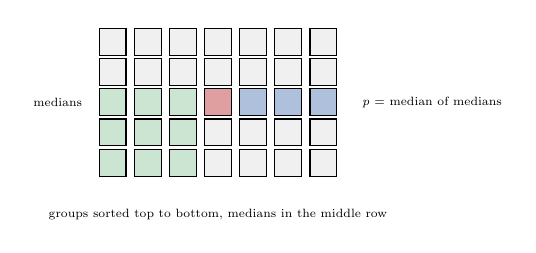
\begin{tikzpicture}[scale=0.62, every node/.style={transform shape}]
    % 7 groups of 5, sorted downward; medians in middle row
    \foreach \g in {0,...,6} {
      \foreach \r in {0,...,4} {
        \ifnum\r=2 \def\fillc{mLightBlue!45}\else\def\fillc{black!6}\fi
        \ifnum\g<3 \ifnum\r>1 \def\fillc{mGreen!30}\fi \fi
        \ifnum\g=3 \ifnum\r=2 \def\fillc{mRed!55}\fi \fi
        \node[draw, minimum size=5.5mm, fill=\fillc] at (\g*0.72, -\r*0.62) {};
      }
    }
    \node[left] at (-0.5,-1.24) {\scriptsize medians};
    \node[below] at (2.16,-3.3) {\scriptsize groups sorted top to bottom, medians in the middle row};
    \node[right] at (5.0,-1.24) {\scriptsize $p$ = median of medians};
  \end{tikzpicture}
  \end{center}

  \begin{block}{Claim}
    At least $\approx \frac{3n}{10}$ elements are $\le p$, and at least $\approx \frac{3n}{10}$ are $\ge p$.
  \end{block}
\end{frame}

\begin{frame}{Proof Sketch}
  There are $\lceil n/5 \rceil$ medians, and at least \alert{half} of them are $\le p$.

  \bigskip
  For each such median, at least \alert{3 of the 5} elements in its group are $\le p$,
  namely the median itself and the two below it.

  \bigskip
  That gives at least
  \[
    3 \left\lfloor \frac{1}{2}\left\lceil \frac{n}{5} \right\rceil \right\rfloor
    \approx \frac{3n}{10}
  \]
  elements $\le p$. Symmetrically for $\ge p$. $\square$

  \bigskip
  \begin{center}
    So the recursive call runs on at most $\approx \dfrac{7n}{10}$ elements.
  \end{center}
\end{frame}

\begin{frame}{The Recurrence}
  \begin{alertblock}{}
    \[
      T(n) = T\!\left(\frac{n}{5}\right) + T\!\left(\frac{7n}{10}\right) + O(n)
    \]
  \end{alertblock}

  \bigskip
  \begin{itemize}
    \item $T(n/5)$: finding the median of the medians (step 3).
    \item $T(7n/10)$: the selection call on $L$ or $G$ (step 4).
    \item $O(n)$: grouping, group medians, and partitioning.
  \end{itemize}

  \bigskip
  \begin{center}
    \small Note $\frac{1}{5} + \frac{7}{10} = \frac{9}{10} < 1$, which is what makes it linear.
  \end{center}
\end{frame}

\begin{frame}{Why It Is $O(n)$}
  \begin{center}
  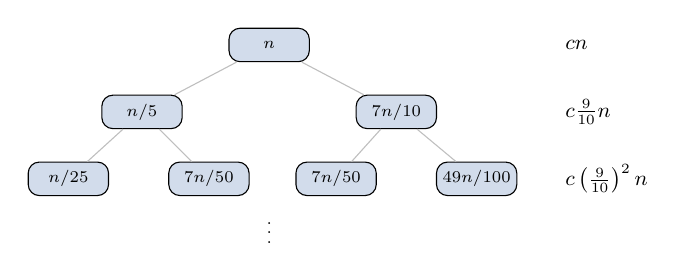
\begin{tikzpicture}[scale=0.85, every node/.style={transform shape},
      lv/.style={draw, rounded corners, fill=mLightBlue!25, minimum width=12mm, minimum height=5mm, inner sep=1pt}]
    \node[lv] (a)  at (0,0)      {\scriptsize $n$};
    \node[lv] (b1) at (-1.9,-1.0) {\scriptsize $n/5$};
    \node[lv] (b2) at (1.9,-1.0)  {\scriptsize $7n/10$};
    \node[lv] (c1) at (-3.0,-2.0) {\scriptsize $n/25$};
    \node[lv] (c2) at (-0.9,-2.0) {\scriptsize $7n/50$};
    \node[lv] (c3) at (1.0,-2.0)  {\scriptsize $7n/50$};
    \node[lv] (c4) at (3.1,-2.0)  {\scriptsize $49n/100$};
    \draw[mGray] (a) -- (b1); \draw[mGray] (a) -- (b2);
    \draw[mGray] (b1) -- (c1); \draw[mGray] (b1) -- (c2);
    \draw[mGray] (b2) -- (c3); \draw[mGray] (b2) -- (c4);
    \node at (0,-2.7) {\scriptsize $\vdots$};
    \node[right] at (4.3,0)    {\small $cn$};
    \node[right] at (4.3,-1.0) {\small $c\frac{9}{10}n$};
    \node[right] at (4.3,-2.0) {\small $c\left(\frac{9}{10}\right)^2 n$};
  \end{tikzpicture}
  \end{center}

  \[
    cn + c\left(\tfrac{9}{10}\right)n + c\left(\tfrac{9}{10}\right)^2 n + \cdots
    = cn \sum_{i=0}^{\infty}\left(\tfrac{9}{10}\right)^i
    = 10cn = O(n).
  \]
\end{frame}

\begin{frame}{Exercise}
  \begin{center}
    What happens with groups of \alert{3} or \alert{7} instead of 5?
  \end{center}

  \bigskip
  Write out the recurrence in each case and decide whether the algorithm is still $O(n)$.
\end{frame}

\begin{frame}{Solution}
  \textbf{Groups of 3.} At least 2 of every 3 elements in half the groups are $\le p$, giving $\approx \frac{2n}{6} = \frac{n}{3}$ on each side, so the recursion is on $\le \frac{2n}{3}$:
  \[
    T(n) = T\!\left(\tfrac{n}{3}\right) + T\!\left(\tfrac{2n}{3}\right) + O(n),
    \qquad \tfrac13 + \tfrac23 = 1.
  \]
  The level work no longer shrinks: every level costs $cn$, and there are $\Theta(\log n)$ of them:
  \alert{$T(n) = \Theta(n \log n)$}.

  \bigskip
  \textbf{Groups of 7.} At least 4 of every 7 in half the groups, giving $\approx \frac{4n}{14} = \frac{2n}{7}$ per side:
  \[
    T(n) = T\!\left(\tfrac{n}{7}\right) + T\!\left(\tfrac{5n}{7}\right) + O(n),
    \qquad \tfrac17 + \tfrac57 = \tfrac67 < 1
    \;\Longrightarrow\; O(n).
  \]

  \begin{center}
    \small Any odd group size $\ge 5$ works; 3 is the one that fails.
  \end{center}
\end{frame}

\begin{frame}[fragile]{Implementation}
  \begin{lstlisting}
function median_of_medians(A, k)
    n = length(A)

    # Base case: sort and return the k-th smallest
    if n <= 10
        return sort(A)[k]
    end

    # Steps 1-2: groups of 5, median of each
    medians = [sort(A[i:i+4])[3] for i in 1:5:n-n%5-4]

    # Step 3: recursively find the median of medians
    p = median_of_medians(medians, (length(medians) + 1) div 2)

    # Step 4: partition and recurse
    L = [a for a in A if a < p]
    E = [a for a in A if a == p]
    G = [a for a in A if a > p]

    if k <= length(L)
        return median_of_medians(L, k)
    elseif k <= length(L) + length(E)
        return p
    else
        return median_of_medians(G, k - length(L) - length(E))
    end
end
  \end{lstlisting}
\end{frame}

\begin{frame}{In Practice}
  \begin{center}
  \begin{tabular}{lll}
    \toprule
                        & worst case      & in practice \\
    \midrule
    Sorting             & $O(n \log n)$   & simple, often fine \\
    Quickselect         & $O(n^2)$        & expected $O(n)$, small constants \\
    Median of medians   & $O(n)$          & large constants \\
    \bottomrule
  \end{tabular}
  \end{center}

  \bigskip
  \begin{center}
    The linear-time guarantee is beautiful, but quickselect with a random pivot
    is usually the faster choice.
  \end{center}
\end{frame}

% =========================================================================
\begin{frame}[standout]
  Questions?
\end{frame}

\end{document}
